%------------------------------------------------------------------
% Einstellen der Grundzüge des Layouts, z. B. Blattgröße
%------------------------------------------------------------------
\documentclass[a4paper,landscape,twoside=false,fontsize=8,numbers=noenddot,DIV=16]{scrreprt}
\usepackage[left=5mm, right=5mm, top=5mm, bottom=5mm]{geometry}
\pagestyle{empty}
%------------------------------------------------------------------
% Importieren den notwendigen packages
%------------------------------------------------------------------
% Packages zum Zeichnen für z. B. Flowchart
\usepackage{tikz}
\usetikzlibrary{shapes,arrows,chains}
\usepackage{verbatim}

% math stuff
\usepackage{amsmath}
\usepackage{amssymb}

% Zum einfügen von mehrseitigen PDFs
%\usepackage{pdfpages}				

% Zum einfügen von Graphen
\usepackage{pgfplots}
\usepackage{pgfplotstable}

% Für das Abkürzungsverzeichnis notwendig
\usepackage[footnote]{acronym}

% Bildumgebungen
\usepackage{graphicx}
\usepackage{float}
\usepackage{xcolor}	

% Literaturumgebungen
\usepackage{cite}					% Zitieren
\usepackage{bibgerm}				% Literatur in Deutscher DIN

% Tabellenumgebung
\usepackage{longtable}				% Tabellen mit Seitenumbruch
\renewcommand\arraystretch{1.4}   		% Tabellen: Zeilen um Faktor x vergrößern
\usepackage{booktabs}				% professionelle Tabellen (Grundeinstellung bei Excel2LaTeX Excel-PlugIn)

% Mathematikumgebungen
%\usepackage{amsmath}
%\usepackage{amssymb}

% Sonstige Umgegebungen
%\usepackage{ifthen}		
%\usepackage{caption}
%\usepackage{subcaption}
\usepackage{listings}
%\usepackage{multirow}
%\usepackage{multicol}		
\usepackage[ngerman]{babel}
\usepackage[latin1]{inputenc}
\usepackage[T1]{fontenc}
	

% Blindtext
\usepackage{blindtext}

% Einstellung des Zeilenabstandes z. B. auf der Titelseite
\usepackage{setspace}

% Für eine Verlinkung im Inhaltsverzeichnis.
% Dieses Paket möglichst als letztes einbinden falls Fehler auftreten!!!
\usepackage{hyperref}
\hypersetup{
    %bookmarks=true,
    unicode=false,
    pdfborder={0 0 0},
    pdftoolbar=true,
    pdfmenubar=true,
    pdffitwindow=false,
    pdfstartview={FitH},
    pdftitle={My title},
    pdfauthor={Author},
    pdfsubject={Subject},
    pdfcreator={Creator},
    pdfproducer={Producer},
    pdfkeywords={keyword1} {key2} {key3},
    pdfnewwindow=true,
    colorlinks=false,
    linkcolor=red,
    citecolor=green,
    filecolor=magenta,
    urlcolor=cyan
}

\usepackage{fancyhdr}
%\usepackage{scrlayer-scrpage}

% Für Hintergrundbilder
\usepackage{eso-pic}



%------------------------------------------------------------------
% Weitere Einstellungen (Farben / Numerierungstiefen)
%------------------------------------------------------------------
%------------------------------------------------------------------
% THI und Continental Farbdefinitionen
%------------------------------------------------------------------
\definecolor{haw_mag}{RGB}{0, 90, 155}
\definecolor{conti}{RGB}{255, 165, 0}
\definecolor{uniFR}{RGB}{0, 76, 153}
\definecolor{gray}{rgb}{0.4,0.4,0.4}
\definecolor{darkblue}{rgb}{0.0,0.0,0.6}
\definecolor{cyan}{rgb}{0.0,0.6,0.6}
\definecolor{pink}  {rgb}{0.67, 0.05, 0.57}
\definecolor{red}   {rgb}{0.87, 0.20, 0.00}
\definecolor{green} {rgb}{0.00, 0.47, 0.00}
\definecolor{violet}{rgb}{0.41, 0.12, 0.61}
\definecolor{blue}  {rgb}{0.21, 0.00, 0.44}
\definecolor{brown} {rgb}{0.39, 0.22, 0.13}


%------------------------------------------------------------------
% Zuweisung der Farben zu den Überschriften
%------------------------------------------------------------------e
\addtokomafont{chapter}{\color{black}}
\addtokomafont{section}{\color{black}}
\addtokomafont{caption}{\color{black}}
\addtokomafont{subsection}{\color{black}}
\addtokomafont{subsubsection}{\color{black}}
\setkomafont{captionlabel}{\color{black}}

%------------------------------------------------------------------
% Tiefe der Numerierung und des Inhaltsverzeichnises:
% Kapitel- bis Unterunterabschnittsüberschriften
%------------------------------------------------------------------
\setcounter{secnumdepth}{4}
\setcounter{tocdepth}{4}




%------------------------------------------------------------------
% Definition einiger globaler Variablen
%------------------------------------------------------------------


%------------------------------------------------------------------
% Dokumentbeginn
%------------------------------------------------------------------
\begin{document}

\setlength{\columnsep}{0.5cm}
\setlength{\columnseprule}{0pt}
\begin{multicols}{3}
	% -----------------------------------------------------------------
% 			  Introduction
% -----------------------------------------------------------------
\begin{tcolorbox}[colback=blue!5!white,colframe=blue!75!black,title=\textbf{Introduction}]
Euklidian Norm: 
\begin{equation*}
{ \parallel x\parallel  }_{ 2 }\quad =\quad \sqrt { \sum _{ i=1 }^{ n }{ { x }_{ i }^{ 2 } }  } \quad =\quad \sqrt { { x }^{ T }x }
\end{equation*}
\begin{equation*}
{\parallel x\parallel  }_{ 2 }^{ 2 } = x^T\cdot x
\end{equation*}
Weighting Eukledian Norm:
\begin{equation*}
{\parallel x\parallel  }_{ Q }^{ 2 } = x^TQ \cdot x
\end{equation*}
Frobenius Norm:
\begin{equation*}
{\parallel x\parallel  }_{ F }^{ 2 } = trace(A{ A }^{ T })=\sum _{ i=1 }^{ n } \sum _{ j=1 }^{ m }{ { A }_{ ij }{ A }_{ ij } } 
\end{equation*}
\begin{equation*}
\triangledown f(x) \quad Jacobian
\end{equation*}
\begin{equation*}
{ \triangledown  }^{ 2 }f(x)\quad Hessian
\end{equation*}
\tcblower
Error in variables
\begin{equation*}
\hat { R } _{ ev }(N)\quad =\quad \frac { \frac { 1 }{ N } \sum _{ k=1 }^{ N }{ u(k) }  }{ \frac { 1 }{ N } \sum _{ k=1 }^{ N }{ i(k) }  }
\end{equation*}
Matrix derivatives
\begin{equation*}
\frac{d(c^Tx)}{dx} = c
\end{equation*} 
\begin{equation*}
\frac{d(x^TAx)}{dx} = (A^T + A)x
\end{equation*} 
Linear and non-linear models:\\
linear if parameters go in linear i.e. ($\theta_1 x^2 + \theta_2 x + \theta_3$), nonliniar if i.e ($\sin(\theta_1)x + \theta_2$) 
\todo[inline]{TODO check that...}

Table of Derivatives:
\begin{center}
\begin{tabular}{|c|c|}
	\hline 
	\textbf{$\mathbf{f(x)}$} & \textbf{$\mathbf{f'(x)}$} \\ 
	\hline 
	$ g(x) \cdot h(x)$& ${\color{red}g'(x)} \cdot h(x) + g(x) \cdot {\color{red}h'(x)}$ \\ 
	\hline 
	$ g(h(x))$ & $g'(h(x)) \cdot h'(x)$ \\ 
	\hline 
	$\sin(x)$ & $-\cos(x)$ \\ 
	\hline 
	$\cos(x)$ & $\sin(x)$ \\ 
	\hline 
	$\tan(x)$& $-\ln(\vert\cos(x))$ \\ 
	\hline 
	$e^{kx}$& $\frac{1}{k}e^{kx} $\\ 
	\hline 
	$\ln(x)$& $\frac{1}{x}$ \\ 
	\hline 
	$\log_ax$& $\frac{1}{\ln a}(x\ln x -x)$ \\ 
	\hline 
\end{tabular} 
\end{center}
\end{tcolorbox}
	% -----------------------------------------------------------------
% 				   Probablility and Statistics
% -----------------------------------------------------------------
\begin{tcolorbox}[colback=cyan!5!white,colframe=cyan!75!black,title=Probablility and Statistics]
Random Variables and Probability
\begin{equation*}
P(A|B) \cdot  P(B) = P(B|A) \cdot  P(A)
\end{equation*}
\begin{equation*}
P(A|B) = \frac { P(A,B) }{ P(B) }  \rightarrow  \frac { P(B,A) \cdot  P(A) }{ P(B) } 
\end{equation*}
\begin{equation*}
P(X \in  [a,b]) = \int _{ a }^{ b }{  p_{ X }(x) dx } 
\end{equation*}
Mean
\begin{equation*}
\mu_X = \mathbb{ E }\{ f(x)\}  := \int _{ -\infty  }^{ \infty  }{  f(x) \cdot  p_{ X }(x) dx } 
\end{equation*}
\begin{equation*}
\mathbb{ E }\{ a + bX\}  := a + b\mathbb{ E }\{ X\} 
\end{equation*}
Variance
\begin{equation*}
\sigma _{ X }^{ 2 } := \mathbb{ E }\{ (X-\mu _{ X })^{ 2 }\}  = \mathbb{ E }\{ X^{ 2 }\} -\mu _{ X }^{ 2 }
\end{equation*}
\begin{equation*}
std dev \, \sigma _{ X } = \sqrt { variance \, \sigma _{ X }^{ 2 } } 
\end{equation*}
\end{tcolorbox}

\begin{tcolorbox}[colback=cyan!5!white,colframe=cyan!75!black,title=Distributions]
Uniform distribution:
\begin{equation*}
{ P_{ y }(x) } = \left\{ \begin{matrix} \frac { 1 }{ b-a }  &  \quad if\quad x  \in  [a,b] \\ 0 & else \end{matrix} \right.
\end{equation*}
Normal (Gaussian) distribution:
\begin{equation*}
p(x) = \frac{1}{\sqrt{2\pi \sigma^2}}\cdot exp(-\frac{(x-\mu)^2}{2\sigma^2})
\end{equation*}
\begin{equation*}
X \sim \mathcal{N}(\mu, \sigma^2)
\end{equation*}
Multidimensional Normal Distribution:
\begin{equation*}
p(x)=\frac { 1 }{ \sqrt { (2\pi )^{ n }\cdot det(\Sigma ) }  } \cdot exp(-\frac { 1 }{ 2 } \, \cdot \, { (x-\mu ) }^{ T }\, \cdot \, \Sigma ^{ -1 }\, \cdot \, (x-\mu )\, )
\end{equation*}
Weibull distribuation: 
\begin{equation*}
F(x) \, = \, 1 - e^{-(\lambda \cdot x)^k}
\end{equation*}
Laplace distribuation:
\begin{equation*}
f(x|\mu,b) = \frac{1}{2b} \cdot exp (-\frac{|x-\mu|}{b})
\end{equation*}
\end{tcolorbox}

\begin{tcolorbox}[colback=cyan!5!white,colframe=cyan!75!black,title=Useful statistic definitions]
Covariance and Correlaton:
\begin{equation*}
\sigma (Y,Z) := \mathbb{E} {(Y-\mu_Y)(Z-\mu_Z)} = 
\end{equation*}
\begin{equation*}
= \int_{-\infty}^{\infty}{\int_{-\infty}^{\infty}{(y-\mu_Y)(z - \mu_Z)\cdot p_{Y,Z} (y,z)\,  dy \, dz} }
\end{equation*}
Covariance Matrix:
\begin{equation*}
\Sigma_x = cov(X) = \mathbb{E}\{XX^T\} - \mu_x \mu^T_x
\end{equation*}
Multidimensional Random Variables:
\begin{equation*}
\mathbb{E}{f(X)} = \int_{\mathbb{R}^n}{f(x)p_X(x) d^n x}
\end{equation*}
\begin{equation*}
cov(X) = \mathbb{E} \{(X-\mu_X)(X-\mu_X)^T\} 
\end{equation*}
\begin{equation*}
cov(X) = \mathbb{E} \{XX^T\} - \mu_X \mu_X^T
\end{equation*}
\begin{equation*}
cov(Y) = \Sigma_y = A \Sigma_x A^T \quad for \quad y = A \cdot x
\end{equation*}
\begin{equation*}
\mathbb{E }\{AX\} =A \cdot \mathbb{ E }\{X\}
\end{equation*}
Rules for variance:
\begin{equation*}
var(X+Y) = var(X)+var(Y)+2 \cdot cov(X,Y)
\end{equation*}
\begin{equation*}
var(aX) = {a}^{2} \cdot var(X)
\end{equation*}
Verschiebesatz:
\begin{equation*}
var(X)={ { \mathbb{E}((X-\mathbb{E}(X)) }^{ 2 } })=\mathbb{E}({ X }^{ 2 })-{ (\mathbb{E}(X)) }^{ 2 }
\end{equation*}

unit Variance is variance = 1

Statistical estimators:\\
\textbf{Biased- and unbiasedness} $\rightarrow$ an estimator ${\hat{\theta}}_{N}$ is called unbiased iff $\mathbb{E}\{ {\hat{\theta}}_{N} ({y}_{N})\} = \theta_0$, where ${\theta}_{0}$ is the true value of a parameter. Otherwise, is called biased.

\textbf{Asymptotic Unbiasedness} $\rightarrow$ An estimator ${\hat{\theta}}_{N}$ is called asymptotically unbiased iff 
$
\lim\limits_{n \to \infty} \mathbb{E}\{ {\hat{\theta}}_{N} ({y}_{N}) \} = \theta_0
$

\textbf{Consistency} $\rightarrow$ An estimator ${\hat{\theta}}_{N} ({y}_{N})$ is called consistent if, for any $ \epsilon > 0$, the probability $
P( {\hat{\theta}}_{N} ({y}_{N}) \in [\theta_0 - \epsilon, \theta_0 + \epsilon])
$ tends to one as $N \rightarrow \infty$.
\end{tcolorbox}

\begin{tcolorbox}[colback=blue!5!white,colframe=blue!75!black,title=Unconstrainded Optimization]
	\begin{description}
		\item[Theorem 1:]{(First Order Necessary Conditions)\\
			If $x^* \in D$ is local minimizer of $f : D \rightarrow \mathbb{R}$ and $f \in C^1$ then
			$\triangledown f (x^*) = 0$
			Definition (Stationary Point) A point $\bar{x}$ with $\triangledown f(\bar{x}) = 0$ is called a stationary point of f.
			}
		\item[Theorem 2:] {(Second Order Necessary Conditions)\\
			If $x^* \in D$ is local minimizer of $f : D \rightarrow R$ and $f \in C^2$ then
			$\triangledown^2 f(x^*) \succeq 0$
			}
		\item[Theorem 3:] {(Second Order Sufficient Conditions and Stability under Perturbations)\\
			Assume that $f : D \rightarrow R$ is $C^2.$ If $x^* \in D$ is a stationary point and
			$ \triangledown^2 f(x^*) \succ 0$
			then $x^*$ is a strict local minimizer of f. In addition, this minimizer is locally unique and is stable against small perturbations of f, i.e. there exists a constant C such that for sufficiently small $p \in \mathbb{R}^n$ holds\\
			\begin{equation*}
			\parallel{x^* - arg\, \underset{x}{min}  (f(x) + p^T x)}\parallel \,\, \leq \, C\parallel{p}\parallel
			\end{equation*}
			}
	\end{description}
\end{tcolorbox}
	% -----------------------------------------------------------------
% 				 Linear Least Squares Estimation
% -----------------------------------------------------------------
asdfdsaf
\begin{tcolorbox}[colback=red!5!white,colframe=red!75!black,title=\textbf{Linear Least Squares Estimation}]
\textbf{Preliminaries:} i.i.d. and Gaussian noise
\begin{flalign*}
	& \textbf{Overall Model: }
	y(k)= \phi (k)^T \theta +\epsilon (k) & \\
	& \textbf{LS cost function as sum: }
	\sum _{k=1}^{N} { (y(k)- \phi(k)^T \theta )}^{2} & \\
	& \textbf{LS cost function: }
	f(\theta )={ \lVert y_N - \Phi_N \theta \rVert }_{2}^{2} & \\
	&\textbf{Unique minimizers: }
	\hat{\theta}_{LS} = \underset{\theta \in \mathbb{R}}{arg\,min} \, f(\theta) \hfil \theta^* = \underbrace{(\Phi^T \Phi)^{-1} \Phi^T}_{\Phi^+} y & \\
	& \textbf{Pseudo Inverse: } \Phi ^+ = (\Phi^T \Phi)^{-1} \Phi^T &
\end{flalign*}
\end{tcolorbox}

\begin{tcolorbox}[colback=red!5!white,colframe=red!75!black,title=\textbf{Weighted Least Squares (unitless)}]
\textbf{For i.i.d noise:} Unweight Least Squares is optimal: $W = I$
\begin{align*}
	f_{WLS}(\theta) &= \sum _{ k=1 }^{ N }\frac {{{ (y(k)-{ \phi (k) }^{ T }\theta )}^{2  } }}{\sigma_{\epsilon}^{2}(k)} = { \lVert y_N - \Phi_N \theta \rVert }_{W}^{2}  \\
	&= { (Y_N - \Phi \cdot \theta ) }^{T} \cdot W \cdot (Y_N - \Phi \cdot \theta )
\end{align*}
\textbf{Solution for WLS: }
\begin{flalign*}
	\hat \theta_{WLS} &= \tilde \Phi^+ \tilde y \qquad 
	\text{ mit } \tilde \Phi = W^{\frac{1}{2}} \Phi \text{ und } \tilde y = W^{\frac{1}{2}} y & \\
	&= \underset{\theta \in \mathbb{R}}{arg\,min} \, f_{WLS}(\theta) = { (\Phi^T W \Phi)}^{-1} \Phi^T Wy
\end{flalign*}
\end{tcolorbox}


\begin{tcolorbox}[colback=red!5!white,colframe=red!75!black,title=\textbf{Ill-Posed Least Squares}]	
\textbf{Singular Value Decomposition: } $A = USV^T \in\mathbb R^{mxn} $
\begin{addmargin}[1em]{0em}
	with $U\in\mathbb R^{mxm}$, $V\in\mathbb R^{nxn}$ and $S\in\mathbb R^{mxn}$ where $S$ is a Matrix with non-negative elements $(\sigma_1,\dots,\sigma_r, 0,\dots,0)$ on the diagonal and 0 everywhere else.
\end{addmargin}
\textbf{Moore Penrose Pseudi Inverse: }
\begin{align*}
	\Phi^+ = VS^+ U^T = V(S^T S+\alpha I)^{-1} S^T U^T
\end{align*}
\hspace{1em} $\Phi^+$ therefore selects $\theta^* \in S^*$ with minimal norm. \\
\textbf{Regularization for Least Squares:}
\begin{align*}
	\underset{a \rightarrow 0}{\lim} (\Phi^T \Phi + \alpha I)^{-1} \Phi^T = \Phi^+ \quad \text{with }\Phi^+ \, MPPI \\
	\theta^* (\alpha )= \underset{\theta \in \mathbb{R}}{arg\,min}  \frac {1}{2} {\rVert y-\Phi\theta \rVert}_{2}^{2} + \frac {\alpha}{2} {\lVert \theta \rVert}_{2}^{2}
\end{align*}
\todo[inline]{Stimmt das auch so mit dem $\alpha$? Ich find das nirgends so.}
\end{tcolorbox}

\begin{tcolorbox}[colback=red!5!white,colframe=red!75!black,title=\textbf{Statistical Analysis of WLS}]
\textbf{Expectation of Least Squares Estimator: }
\begin{align*}
	E \{\hat \theta_{WLS} \} = E \{ {(\Phi_{N}^{T} W \Phi_N)}^{-1} \Phi_{N}^{T} W y_N \} = \theta_0
\end{align*}
\textbf{Covariance of the least squares estimator: }
\begin{align*}
	cov(\hat \theta_{WLS}) &= {(\Phi_{N}^{T} W \Phi_N)}^{-1} = {(\Phi_{N}^{T} \Sigma_{\in N }^{-1} \Phi_{N}) }^{-1} \\
	cov(\hat \theta_{WLS}) &\succeq {(\Phi_{N}^{T} W \Phi_{N})}^{-1}
\end{align*}
\end{tcolorbox}

\begin{tcolorbox}[colback=red!5!white,colframe=red!75!black,title=\textbf{Example LLS}]
\textbf{Example of the Linear Least Square Estimator for: $N=2$}
\begin{equation*}
	\varepsilon(1) \sim \mathcal{N}(0|{\sigma}^{2}_{1}) \hfil \varepsilon(2) \sim 	\mathcal{N}(0|\sigma^{2}_{2})
\end{equation*}

\begin{flalign*}
	& N=2; \quad \Sigma_{\varepsilon_{N}} = 
	\begin{bmatrix} \sigma_{1}^{2} & 0 \\ 0 & \sigma_{2}^{2} \end{bmatrix} 
	\qquad
	W^{OPT} = \Sigma_{\varepsilon_N}^{-1} = 
	\begin{bmatrix} \frac {1}{\sigma_{1}^{2}}  & 0 \\ 0 & \frac {1}{\sigma_{2}^{2}}  \end{bmatrix} &
\end{flalign*}

\begin{flalign*}
	cov(\hat \theta_{WLS}) &= {(Y_N - \Phi_N \theta)}^T \cdot W \cdot (Y_N - \Phi_N \theta ) & \\
	&= \sum_{k=1}^{2} (y(k) - \phi(k)^T \theta ) \cdot \frac {1}{\sigma_{k}^{2}} \cdot (y(k) - \phi(k)^T \theta) &
\end{flalign*}

\textbf{Measuring the goodness of Fit using:  ${R}^{2}$} \quad ($0\le {R}^{2} \le1$)
\begin{align*}
R^2 &= 1 - \frac{ { \lVert y_N - \Phi_N \hat \theta \rVert}_{2}^{2} }{ {\lVert y_N \rVert}_{2}^{2} } = 1 - \frac{ {\lVert \epsilon_N \rVert}_{2}^{2} }{ {\lVert y_N \rVert}_{2}^{2} } \\
&= \frac{ {\lVert y_N \rVert}_{2}^{2} - {\lVert \epsilon_N \rVert}_{2}^{2} }{ {\lVert y_N \rVert}_{2}^{2} } = \frac{ {\lVert \hat y_N \rVert}_{2}^{2} }{ {\lVert y_N \rVert}_{2}^{2} }
\end{align*}
Residual: $ \epsilon_N \uparrow \rightarrow \quad R^{2} \rightarrow 0 \,\,(\Rightarrow bad)$
\tcblower
\textbf{Estimating the Covariance with the Single Experiment: }
\begin{flalign*}
\hat \sigma_{\varepsilon}^{2} &:= \frac{1}{N-d} \sum_{k=1}^{N} (y(k)-\phi(k)^T \hat \theta_{LS})^2 = \frac{ {\lVert y_N - \phi_N \hat \theta_{LS} \rVert}_{2}^{2} }{ N-d } &\\
\hat \Sigma_{\hat \theta} &:= \hat \sigma_{\varepsilon}^{2} (\phi^{T}_{N} \phi_{N})^{-1} = \frac{ {\lVert y_N -\phi_N \hat \theta_{LS} \rVert}_{2}^{2} }{ N-d } \cdot (\phi^{T}_{N} \phi_{N})^{-1} &
\end{flalign*}
\end{tcolorbox}

	% -----------------------------------------------------------------
% 				 Maximum Likelihood Estimation
% -----------------------------------------------------------------
\begin{tcolorbox}[colback=yellow!5!white,colframe=yellow!75!white,coltitle=black,title=\textbf{Bayesian Estimation and the Maximum a Posteriori Estimate}]
	
	\textbf{Assumptions:}
	\begin{itemize}
		\item[-] Measurement: \quad $y_N \in \mathbb{R}^N$ \quad has i.i.d. noise	
		\item[-] Linear Model: \quad $M(\theta) = \phi_N \cdot \theta$ \quad and $\theta \in \mathbb{R}$
	\end{itemize}
	\begin{flalign*} 
	p(\theta |y_N) &= \frac{p(y_N,\theta)}{p(y_N)} = \frac{ p(y_N | \theta) \cdot p(\theta) }{ p(y_N) } &\\
	\hat{\theta}_{MAP} &= \underset{\theta\in \mathbb{R}}{\text{arg\,min}} \{ -\log (p (y_N| \theta) ) -\log (p(\theta))\}
	\end{flalign*}
	
	\textbf{MAP Example:} Regularised Least Squares
	\begin{flalign*}
	\theta &= \bar \theta \pm \sigma_\theta \quad \text{with} \quad \bar \theta =  \theta_{\text{a-priori} } &\\
	\hat \theta_{MAP} &= \underset{\theta \in \mathbb{R}}{\text{arg\,min}} \frac{1}{2} \cdot \frac{1}{\sigma_{\epsilon^2 }} \cdot \lVert y_N - \Phi_N \cdot \theta \rVert_{2}^{2} + \frac{1}{2} \cdot \frac{1}{\sigma_{\theta}^2} \cdot (\theta - \bar \theta)^2
	\end{flalign*}
\end{tcolorbox}

\begin{tcolorbox}[colback=yellow!5!white,colframe=yellow!75!white,coltitle=black,title=\textbf{Maximum Likelihood Estimation}]
\textbf{$L_2$ Estimation: Maximum Likelihood Estimation (ML)}:
\begin{itemize}
	\item[-] Measurement Errors assumed to be Normally distributed
	\todo[inline]{Ist das wirklich so ? Jo, L2 -> Gaussian oder?}
	
	\item[-] Model described by a non-linear function M(\(\theta\))
	
	\item[-] Every unbiased estimator needs to satisfy the Cramer-Rau inequality, which gives a lower bound on the covariance matrix
\end{itemize}

\begin{flalign*}
	& \textbf{Model: } y = M(\theta) + \epsilon \qquad  &\\
	& P(y|\theta ) = C \prod_{i=1}^{N} exp \left(\frac{-(y_i - M_i (\theta))^2}{2\cdot \sigma_{i}^{2}}\right) \quad 
	C = \prod_{i=1}^{N} \frac{1}{\sqrt{2\cdot \pi \sigma_{i}^2 } }&
\end{flalign*}
\textbf{Positive log-Likelihood: } \text{\small Logarithm makes a product to a sum!}
\begin{align*}
	\log p(y|\theta) = \log(C) + \sum_{i=1}^{N} -\frac{(y_i - M_i (\theta ))^2}{2 \cdot \sigma_{i}^2} 
\end{align*} 
\textbf{Negative log-Likelihood:}
\begin{flalign*}
	& \hat \theta_{ML} = \underset{\theta \in \mathbb{R}^d}{arg\,max} \  p(y|\theta ) = \underset{\theta \in \mathbb{R}^d}{\text{arg\,min}} \sum_{i=1}^{N} \frac{(y_i - M_i (\theta))^2}{2 \sigma_{i}^{2}} & \\
	& = \underset{\theta}{\text{arg\,min}} \frac{1}{2} \sum_{i=1}^{N} \left(\frac{y_i - M_i (\theta)}{\sigma_i }\right)^2 & \\
	& = \underset{\theta \in \mathbb{R}^d}{\text{arg\,min}} \frac{1}{2} \lVert S^{-1} (y - M(\theta) )\rVert_{2}^{2} \qquad
	\text{mit: } S = \begin{bmatrix} \sigma_{ 1 } & & \\ & \ddots & \\	& & \sigma_{ N } \end{bmatrix}&
\end{flalign*}

\textbf{$L_1$ Estimation:}
\begin{itemize}
	\item[-] Measurement Errors assumed to be Laplace distributed and more robust against outliers.
\end{itemize}
\begin{flalign*}
	 \underset{\theta}{min} \lVert y-M(\theta) \rVert_1 &= \underset{\theta}{min} \sum_{i=1}^{N} |y_i - M_i (\theta) | & \\
	& \Rightarrow \text{ median of } \{ Y_1, \cdots, Y_N \} &
\end{flalign*}
\end{tcolorbox}

\begin{tcolorbox}[colback=yellow!5!white,colframe=yellow!75!white,coltitle=black,title=\textbf{Recursive Linear Least Squares}]
\begin{flalign*}
	\theta_{ML}(N) &= \underset{\theta \in \mathbb{R}}{\text{arg\,min}} \frac{1}{2} \lVert y_N - \Phi_N \cdot \theta \rVert_{2}^{2} \qquad \text{(forgetting factor: } \alpha )&\\
	\hat \theta_{ML} (N+1) &= \underset{\theta \in \mathbb{R}^d}{\text{arg\,min}} \left(\alpha \cdot \frac{1}{2} \cdot \lVert \theta - \hat \theta_{ML}(N) \rVert Q_N^2 \right. & \\
	&\quad \left. + \frac {1}{2} \cdot \lVert y(N+1) - \varphi (N+1)^T \cdot \theta \rVert_{2}^{2} \right) & \\
	& Q_0 \quad \text{given, and} \quad \hat{ \theta } _{ML}(0) \quad \text{given} & \\
	Q_{ N+1 } &= \alpha \cdot Q_N + \varphi (N+1) \cdot  \varphi (N+1)^{T} & \\
	\hat \theta_{ML}(N+1) &= \hat \theta_{ML}(N)+Q_{N+1}^{-1} \cdot  \varphi (N+1) & \\ 
	& \quad \cdot [y(N+1) - \varphi(N+1)^T  \cdot \hat{ \theta }_{ML}(N)] &
\end{flalign*}
\end{tcolorbox}

\begin{tcolorbox}[colback=yellow!5!white,colframe=yellow!75!white,coltitle=black,title=\textbf{Cramer-Rao-Inequality (Fisher information Matrix M)}]
$
\Sigma_{\hat{\theta}} \succeq M^{-1} = (\Phi^T_N \cdot \Sigma^{-1} \cdot \Phi)^{-1} \quad
M = \int_{y_n}\nabla^2_{\theta} L(\theta_0, y_n) \cdot p(y_n \vert \theta_0) dy_n
$
\textbf{Assumptions:}
\begin{itemize}
	\item[-] Minimising a Linear Model
	\item[-] Gaussian Noise: $X \sim \mathcal{N}(0, \Sigma))$
\end{itemize}

\begin{flalign*}
	L(\theta ,y_N) &= - \log (p(y_N | \theta)) & \\
	& = \frac{1}{2} \cdot (\Phi_N \cdot  \theta - y_N)^T \cdot \Sigma^{-1} \cdot (\Phi_N  \cdot \theta - y_N) & \\
	M &= \mathbb{E} \{\nabla^2_\theta \, L( \theta ,y_N)\}  = \nabla^2_\theta  L(\theta ,y_N) = \Phi_N^T \cdot \Sigma^{-1} \cdot \Phi_N & \\
 &\Rightarrow W = \Sigma^{-1} \text{ is the optimal weighting Matrix for WLS.} &
\end{flalign*}
\end{tcolorbox}
	% -----------------------------------------------------------------
%		 				 Dynamic Models
% -----------------------------------------------------------------

\begin{tcolorbox}[colback=green!5!white,colframe=green!75!black,title=\textbf{Continuous Time Systems}]
	\textbf{Ordinary Differential Equations (ODE):}
	\begin{align*}
	\dot{ x } &= f( x(t), u(t), \epsilon(t), p)
	\end{align*}
	
	\textbf{Differential Algebraic Equations(DAE):}
	\begin{align*}
	\dot{ x } &= f( x(t), u(t), \epsilon(t), p)\\
	0 &= g(x, z).
	\end{align*}
	
	\textbf{LTI Sytem (ODE):}
	\begin{align*}
	\dot x &= Ax+Bu \quad y = Cx+Du \\
	G(s) &= C (sI-A)^{-1} B+D
	\end{align*}
\end{tcolorbox}


\begin{tcolorbox}[colback=green!5!white,colframe=green!75!black,title=\textbf{Numerical Integration Methods}]
	
	\textbf{Euler Integration Step}
	\begin{align*}
	\tilde{x}(t; x_{init}, u_{const}) &= x_{init} + t f(x_{init}, u_{const}), \quad t \in [0, \Delta t]\\
	\tilde{x}_{j+1} &= \tilde{x}_j + h f (\tilde{x}_j, u_{const}), \quad j = 0, ..., M - 1
	\end{align*}
	\begin{itemize}
		\item[-] Approximation becomes better by decreasing the step size h.
		\item[-] Concistency Error: $h^2$
		\item[-] Total Number of steps: $\Delta t / h$
		\item[-] Error in the final step of order $h \Delta t$
		\item[-] Linear in step size $\rightarrow$ order one
		\item[-] Taking more steps is more accurate but needs more computional time
	\end{itemize}
	
	\textbf{Runge-Kutta Method of Order Four}
	\begin{align*}
		k_1 &= f(\tilde{x}_j, u_{const})\\
		k_2 &= f(\tilde{x}_j, \frac{h}{2} k_1, u_{const})\\
		k_3 &= f(\tilde{x}_j, \frac{h}{2} k_2, u_{const})\\
		k_4 &= f(\tilde{x}_j, h k_3, u_{const})\\
		\tilde{x}_{j+1} &= \tilde{x}_j + \frac{h}{6} (k_1 + 2k_2 + 2k_3 + k_4)
	\end{align*}
	
	One Step of RK4 is thus as expensive as four steps of euler\\
	accurency of final approximation is of order $h^4 \Delta$ t\\
	$\rightarrow$ rk4 needs fewer functions to obtain the same accuracy level as euler
\end{tcolorbox}

\begin{tcolorbox}[colback=green!5!white,colframe=green!75!black,title=\textbf{Discrete Time Systems}]
	\begin{tabular}{ll}
		Det. Model as State Space  & Stoch. Model as State Space  \\
		Det. Model as Input-Output  & Stoch. Model as Input-Output 
	\end{tabular}

	\textbf{State Space Model}\\
	$ x_{k+1} = f_k(x_k,u_k), k = 0,1,\dots,N-1$ with input vector $u_k$ and state vector $x_k$
	
	\textbf{Input-Output Model}\\
	$y(k) = h(u(k),\dots,u(k-n),y(k-1),\dots,y(k-n))$
	\\
	
	\textbf{LTI system as State-Space Model:}
	\begin{align*}
	x_{k+1} = A x_k + B u_k, \quad k = 0, 1,..., N - 1. 
	\end{align*}

	\textbf{LTI system as Input-Output Model:}
	\begin{flalign*}
	G(s) &= \frac{ b_0 + b_1s+...+b_ns^n }{ a_0+a_1s+...+a_{n-1}s^{n-1}+s^n } \quad | \cdot s = z^{-1} &\\
	G(z) &= \frac{ b_0 + b_1 z^{-1}+...+b_n z^{-n} }{a_0+a_1z^{-1}+...+a_n z^{-n}} &\\
	&= \frac{ b_0z^n+b_n z^{n-1}+...+b_n}{a_0 z^n+a_1 z^{n-1}+...+a_n} \quad \Rightarrow \text{Also called "polynomial model".} &
	\end{flalign*}	
\end{tcolorbox}		
\begin{tcolorbox}[colback=green!5!white,colframe=green!75!black,title=\textbf{Deterministic Model}]
	The output of the system can be obtained with absolute certainty. The Output $y$ or the state x, depend on the known inputs $u(1), \dots, u(N)$, the previous Outputs $y(1), \dots, y(N)$ or state $x(n-1)$ and initial conditions.  
	\textbf{State Space Model}
	\begin{align*}
	x(t+1) = f(x(k), u(k))\\
	y(k) = g(x(k), u(k))
	\end{align*}
	Initial conditions: $x(1) = x_{init}$
	
	\textbf{Input-Output Model}
	\begin{align*}
	y(k) &= h(u(k), ..., u(k-n), y(k-1), ..., y(k-n))\\
	\end{align*}
	Initial conditions: $y(1) = y_1,\dots,y(n) = y_n  \;\; u(1)= u_1,\dots,u(n) = u_n$
	
	
	\textbf{Finite Impulse Response (FIR): } 
	\begin{align*}
		y(k) &= b_0 u(k) + ... + b_{n_b} u(k-n_b) \\
		G(z) &= b_0 + b_1z^{-1} + ... + b_{n_b}z^{-n_b} \quad | \cdot \frac{z^{n_b}}{z^{n_b}} \\
		&= \frac{b_0 z^{n_b} + b_1 z^{ n_{b-1} } + ... + b_{n_b} }{z^{n_b}}
	\end{align*}
	
	\textbf{Auto Regressive Models with Exogenous Inputs (ARX): }
	\begin{align*}
		a_0y(k)+\dots+a_{n_a}y(k-n_a) = b_0u(k) + \dots+b_{n_b}u(k-n_b)\\
	\end{align*}
	\begin{align*}
	G(z) = \frac{b_0z^n + b_1z^{n-1} + \cdots + b_n}{a_0z^n + a_1z^{n-1} + \cdots + a_n}
	\end{align*}
	The next output depends on the previous output. Also called \textbf{IIR} (infinite impulse response)
	
\end{tcolorbox}		
\begin{tcolorbox}[colback=green!5!white,colframe=green!75!black,title=\textbf{Stochastic Model}]
	Real systems are far from deterministic. 
	\begin{itemize}
		\item there is stochastic noise $\epsilon(k)$ 
		\item there are constant and unknown parameters $p$
		\item measured outputs depend $y(k)$ depend in both, $\epsilon(k)$ and $p$ 
	\end{itemize}
	
	Assumptions:  noise is \textbf{i.i.d} and enters the model like a normal input, but as a random variable\\
	
	\textbf{State Space Model}
	\begin{align*}
	x(t+1) = f(x(k), u(k), \epsilon(k)) \\
	y(k) = g(x(k), u(k), \epsilon(k))
	\end{align*}
	
	\textbf{Input-Output Model}
	\begin{align*}
	y(k) &= h(u(k), ..., u(k-n), y(k-1), ..., y(k-n), \epsilon(k), ..., \epsilon(k-n))\\
	\text{for} \quad k &= n + 1, n + 2, ...
	\end{align*}	
	
	\textbf{Measurement Noise (Output Error Model)}
	\begin{align*}
	y(k) = M(k; U, x_{init}, p) + \epsilon(k)
	\end{align*}
	\tcblower
	\section*{Stochastic Disturbance (Equation Errors)}
	\begin{align*}
	y(k) &= h(p, u(k), ..., u(k-n), y(k-1), ..., y(k-n)) + \epsilon(k)\\
	for \quad k& = n + 1, n + 2, ...
	\end{align*}
	
	\textbf{Linear In the Parameters models (LIP):}
	\begin{align*}
	y(k) &= \sum_{ i = 1}^{d}\theta_i\phi_i(u(k)...,y(k-1),...)+\epsilon(k)\\
	y(k) &= \varphi(k)^T\theta + \epsilon(k) \quad \text{where} \, \varphi = (\phi_1(\cdot),... ,\phi_d(\cdot)) 
	\end{align*}

	\textbf{LIP-LTI Models with Equation Errors (ARX)}\\
	combining best of two worlds (LTI and LIP)
	\begin{align*}
	a_0y(k) + ...+a_{n_{a}}y(k-n_a) = b_0u(k) + ... + b_{n_{b}}u(k-n_b) + \epsilon(k)
	\end{align*}
	
	\textbf{Auto-regressive moving average with eXogeneous input (ARMAX):}
	\begin{align*}
	a_0y(k) + ... + a_{n_a}y(k-n_a)\\
	=\\
	b_0u(k) + ... + b_{n_b} u(k - n_b) + \epsilon(k) + c_1 \epsilon(k-1) + ... + c_{n_x} \epsilon(k-n_c)
	\end{align*}
	
	\textbf{Auto-regressive moving average without inputs (ARMA):}
	\begin{align*}
	a_0y(k) + ... + a_{n_a}y(k-n_a)\\
	=\\
	\epsilon(k) + c_1 \epsilon(k-1) + ... + c_{n_x} \epsilon(k-n_c)
	\end{align*}
	Where $c_i$ represent the noise coefficient
	Have to use non-linear leas squares with the unknown noise terms$ \epsilon(k-i)$
	
	\textbf{Difference Deterministic and Stochastic Models}
	\begin{align*}
	- &stochastic noise \epsilon(k)\\
	- &unknown but constant parameter p\\
	- &measured output y(k) depend on both, \epsilon(k) and p
	\end{align*}
\end{tcolorbox}

\begin{tcolorbox}[colback=green!5!white,colframe=green!75!black,title=\textbf{Example for State Space Model}]
	$\ddot{a} = m \cdot \dot{a} + g\cdot a + c \cdot u$\\
	$y = \dot{a}$\\
	$x = \begin{bmatrix}
		a \\ \dot{a}
	\end{bmatrix}$
	$
	\dot{x} = \begin{bmatrix}
	\dot{a} \\ \ddot{a}
	\end{bmatrix}
	$
	$ \dot x = Ax+Bu \quad y = Cx+Du $
	\\
	$
	A = \begin{bmatrix}
	0 & 1 \\
	g & m \\
	\end{bmatrix}
	$
	$ B= \begin{bmatrix}
	0 \\
	c
	\end{bmatrix}$
	$C = \begin{bmatrix}
	0 & 1
	\end{bmatrix} $
	$D = \begin{bmatrix}
	0
	\end{bmatrix}$
	\todo[inline]{check it}
\end{tcolorbox}

\begin{tcolorbox}[colback=purple!5!white,colframe=purple!75!black,title=\textbf{Pure Output Error (OE) Minimization}]
	Assume: i.i.d. gaussian noise only affecting output\\
	using non-linear least squares
	\begin{align*}
	\theta_{ML} =\underset{\theta}{\text{min}} \sum_{k=1}^{N} (y(k)-M(k;U, x_{init} p))^2
	\end{align*}
	
	\textbf{Output Error Minimization for FIR Models:}
	lead to convex problems, therefore global minimum can be found
	\begin{flalign*}
	y(k) &= (u(k), u(k-1), ..., u(k-n_{n_b})) \cdot \theta +\varepsilon(k) &\\
	&= \underset {\theta}{ \text{min} } \sum_{k=n_{b}+1}^{N} (y(k)-\underbrace{(u(k), u(k-1),... , u(k-n_{n_b}))}_{\text{Deterministic part is also}\, M(k; U, x_{init}, p)} \cdot \theta)^2 &
	\end{flalign*}
	
	They often need a very high dimension $n_b$ to obtain a reasonable fit. As a consequence ARX models are usually used instead.
	
	\textbf{Equation Error Minimization:}
	Assume: i.i.d. $\epsilon(k)$ noise enters the input-output equation as additive disturbance
	
	\begin{align*}
	y(k) &= h(p, u(k), ..., u(k-n), y(k-1), ..., y(k-n)) + \epsilon(k)\\
	\text{for} \quad k &= n + 1, n + 2
	\end{align*}
	
	if the i.i.d noise is gaussian, a maximum likelihood formulation to estimate the unknown parameter vector $\theta = p$ is given:
	
	\begin{align*}
	\theta_{ML} = \underset {\theta}{ \text{min} } \sum_{k = n + 1}^{N}{(y(k) - h(p, u(k), ..., y(k-1), ...)) )^2}
	\end{align*}
	u and k are known input and output measurements, and the algorithm minimises the so called \textbf{equation errors} or \textbf{prediction errors}.
	
	This problem is also known as \textbf{Prediction error minimisation(PEM)}
	Such a problem is convex if $p$ enters linearly in $f$, i.e. if the model is \textbf{linear-in-the-parameters (LIP)}
	
	
	
	\textbf{PEM of LIP Models}
	
	\begin{align*}
	y(k) &= \varphi(k)^T\theta + \epsilon(k)\\
	\quad \text{where} \, \varphi &= (\phi_1(\cdot),... ,\phi_d(\cdot))^T \text{are the regressor variables}
	\end{align*}
	
	considering this last expression, the prediction error minimisation(PEM) problem can be formulated as:
	
	\begin{align*}
	\underset{\theta}{\text{min}} \underbrace{\sum_{k=1}^{N} (y(k)-\varphi(k)^\text{T} \theta)^2}_{= \parallel y_N - \Phi_N \theta \parallel_2^2}
	\end{align*}
	Which can be solved using LLS $\theta^* = \Phi^+_N y_N$
	
	\textbf{Special Case: PEM of LIP-LTI Models with Equation Errors(ARX)}
	General ARX model equation
	\begin{align*}
	a_0y(k)+...+a_{n_{a}}y(k-n_a) = b_0u(k)+...+b_{n_{b}}u(k-n_b)+\epsilon(k)
	\end{align*}
	
	In order to have a determined estimation problem, $a_0$ has to be fixed, otherwise the number of optimal solutions would be infinitive. Therefore we sually fix $a_0 = 1$ and use $\theta = (a_1, ..., a_{n_a}, b_0, ..., b_{n_b})^\text{T}$ as the parameter estimation vector. The regressor vector is given by:
	\begin{align*}
	\varphi = (-y(k-1), ..., -y(k-n_a), u(k), ..., u(k-n_b))^\text{T}
	\end{align*}
	leading to the optimal solution provided by LLS:
	\begin{align*}
	y(k) = \varphi(k)^\text{T} \theta + \epsilon(k)
	\end{align*}
	
\end{tcolorbox}
\begin{tcolorbox}[colback=purple!5!white,colframe=purple!75!black,title=\textbf{Pure Output Error (OE) Minimization}]
	\textbf{Models with Input and Output Errors:}
	
	\begin{align*}
	y(k)=M(k;U + \varepsilon_{N}^{u}, x_{init}, p) + \epsilon^y(k)
	\end{align*}
	
	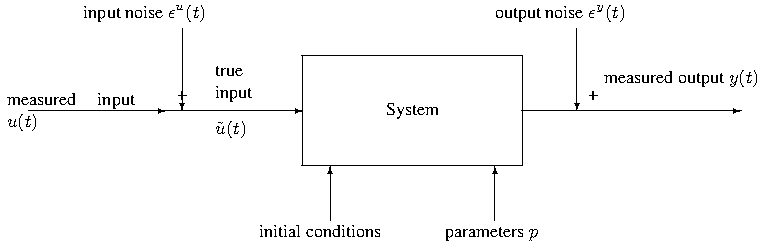
\includegraphics[width=\textwidth]{model.pdf}
	
	Assume: i.i.d. gaussian noise on both input and output with variance $\sigma_u^2$ for the input and $\sigma_y^2$ for the output
	
	\begin{align*}
	& \underset{\theta}{arg\,min} \sum_{k-1}^{N} \frac{1}{\sigma_{y}^{2}} (y(k)-M(k;U+ \epsilon_{N}^{u},x_{init},p))^2 + \frac{1}{\sigma_{u}^{2}} (\epsilon_u (k))^2 & \\
	& \underset{\theta}{arg\,min} \sum_{k-1}^{N} \frac{1}{\sigma_{y}^{2}} (y(k)-M(k;\tilde U, x_{init}, p))^2 + \frac{1}{\sigma_{u}^{2}} (u(k)-\tilde u(k) )^2 &
	\end{align*}
	
	
\end{tcolorbox}

	% -----------------------------------------------------------------
%	 Non parametric and frequency domain identification methods
% -----------------------------------------------------------------
\section*{Fourier Transformation}
\textbf{How to compute FT?} By DFT, which solves the problem of finite time and discrete values.

\textbf{Can we use an input with many frequencies to get many FRF (Frequency Response Function) values in a single experiment?} So far only frequency sweeping (high comp. times due to repetition for each frequency). We should use multisines!

\section*{Aliasing and Leakage Errors}
\begin{description}
\item[Aliasing Error] due to sampling of continous signal to discrete signal. Avoid with Nyquist Theoreme:

\begin{equation*}
f_{Nyquist} = \frac{1}{2\Delta t} [Hz] \quad or \quad \omega_{Nyquist} = \frac{2 \pi }{ 2\Delta t} [rad/s]
\end{equation*}

\item[Leackage Error] due to windowing.
\begin{equation*}
\omega _{ base }:=\frac { 2\pi  }{ N\cdot \Delta t } =\frac { 2\pi  }{ T }  \rightarrow \omega = m\frac { 2\pi  }{ N\cdot \Delta t }
\end{equation*}
\end{description}


\section*{Crest Factor = Scheitelfaktor}
\begin{equation*}
CrestFactor=\frac { u_{ max } }{ u_{ rms } } \quad with:
\end{equation*}
\begin{equation*}
u_{ rms }\, := \sqrt{ \frac { 1 }{ T } \int _{ 0 }^{ T }{ u(t)^2 \, dt }  } \quad and \quad u_{ max }\, :=\underset { t\, \in \, [0,T] }{ max } |u(t)|
\end{equation*}

\section*{Optimising Multisine for optimal crest factor}
\begin{description}
\item[Frequency:] Choose frequencies in logarithmic manner as multiples of the base frequency. $\qquad \omega_{k+1}/\omega_{k} \approx 1.05$
\item[Phase:] To prevent high peaks (Crest Factor) in the Signal, the phases of the different frequencies are modulated accordingly. (Positive interference)
\end{description}


\section*{Multisine Identification Implementation procedure}
\begin{description}
\item[Window Length] integer multiple of sampling time:  \( T = N \cdot \delta t\)
\item[Harmonics of base frequency] are contained in multisine \\ \( {\omega}_{base} = \frac{2 \pi}{T}\)
\item[Highest contained Frequency] is \textbf{half} of Nyquist frequency: \( {\omega}_{Nyquist}  = \frac{2 \pi}{4 \Delta T}\)

\item[Experiment and Analysis] (step 2): Insert Multisine periodically. Drop first Periods (till transients died out). Record M Periods, each with N samples, of input and output data. Average all the M periods and make the DFT (or vice versa). Finally build transfer function.
\end{description}

\begin{equation*}
{\hat{G} _{j{\omega}_{k}}}=\frac{\hat{Y}(k(p))}{\hat{U}(k(p))}
\end{equation*}





\section*{Nonparametric and Frequency Domain Identification Models}
Impulse response and transfer function

\begin{equation*}
y(t)=\int _{ 0 }^{ \infty  }{ g(\tau)u(t-\tau) \delta t } 
\end{equation*}

\begin{equation*}
Y(s)=G(s)\cdot U(s)
\end{equation*}

\begin{equation*}
G(s)=\int _{ 0 }^{ \infty  }{ \epsilon }^{ -st }g(t)dt
\end{equation*}

Bode diagram from frequency sweeps
\begin{equation*}
u(t)=A\cdot sin(\omega \cdot t),\quad y(t)=\parallel G(j\cdot \omega )\parallel A\cdot sin(\omega \cdot t+\alpha )
\end{equation*}


\section*{Online estimation for dynamic systems}
\subsection*{Recursive Least Squares}
New Inverse Covariance:
\begin{equation*}
Q_K \, = \, Q_{k-1} + \phi_K\,\phi_K^T
\end{equation*}
Innovation update:
\begin{equation*}
\hat { \theta  } _{ k }\, =\, \hat { \theta  } _{ k-1 }+\underset { ``innovation'' }{ \underbrace { Q_{ k }^{ -1 }\, \phi _{ k }\, (y_{ k }\, -\, \phi _{ k }^{ T }\, \hat { \theta  } _{ k-1 }) }  } 
\end{equation*}
General Optimization Problem:
\begin{equation*}
\hat { \theta  } _{ k }\, =\, arg\, \underset { \theta  }{ min } \, (\theta -\hat { \theta  } _{ 0 })^{ T }\cdot Q_{ 0 }\cdot (\theta -\hat { \theta  } _{ 0 })+\sum _{ i=1 }^{ k }{ (y_k-\phi_k^T\ \, \cdot \, \theta)^2 } 
\end{equation*}

\section*{Kalman Filter}
Valid for Discrete and Linear!\\
(If recursive least squares: \( x_{ k+1 }\, =\, A_{ k }\cdot x_{ k } \)
\begin{equation*}
x_{ k+1 }\, =\, A_{ k }\cdot x_{ k }+\omega _{ k }\quad and\quad y_{ k }=C_{ k }\cdot x_{ k }+v_{ k }
\end{equation*}
\subsection*{Steps of Kalman Filter}
\begin{description}
\item[1 Prediction] $\hat { x } _{ [k\, |\, k-1] }\, =\, A_{ k-1 }\cdot \hat { x } _{ [k-1\, |\, k-1] }\\ P_{ [k\, |\, k-1] }\, =\, A_{ k-1 }\cdot { P }_{ [k-1\, |\, k-1] }\, \cdot \, A_{ k-1 }^{ T }\cdot { W }_{ k-1 }$ \\
if recursive linear least squares without \( { W }_{ k-1 } \).
\item[2 Innovation update] $P_{ [k\, |\, k] }\, =\, (P_{ [k\, |\, k-1] }^{ -1 }+C_{ k }^{ T }\, \cdot \, { V\,  }^{ -1 }\, \cdot \, C_{ k })^{ -1 }\\ \hat { x } _{ [k\, |\, k] }\, =\, \hat { x } _{ [k\, |\, k-1] }+P_{ [k\, |\, k] }\, \cdot \, C_{ k }^{ T }\, \cdot \, { V\,  }^{ -1 }\, \cdot \, (y_{ k }-C_{ k }\, \cdot \, \hat { x } _{ [k\, |\, k-1] })$
\end{description}

\subsection*{Bode Diagram:}
Magnitude = Amplitude $|G(j\omega)|$\\
Phase $arg \, G(j\omega)$
\end{multicols}

\end{document}
